\documentclass[review]{elsarticle}

%% Use the option review to obtain double line spacing
%% \documentclass[authoryear,preprint,review,12pt]{elsarticle}

%% Use the options 1p,twocolumn; 3p; 3p,twocolumn; 5p; or 5p,twocolumn
%% for a journal layout:
%% \documentclass[final,1p,times]{elsarticle}
%% \documentclass[final,1p,times,twocolumn]{elsarticle}
%% \documentclass[final,3p,times]{elsarticle}
%% \documentclass[final,3p,times,twocolumn]{elsarticle}
%% \documentclass[final,5p,times]{elsarticle}
%% \documentclass[final,5p,times,twocolumn]{elsarticle}

\usepackage{hyperref}
\usepackage{amsmath}
\usepackage{amssymb}
\usepackage{braket}
\usepackage{siunitx}
\usepackage[version=4]{mhchem}
\usepackage{tikz}
\usetikzlibrary{positioning}
\usetikzlibrary {arrows.meta} 
\usepackage{paralist}

%% The lineno packages adds line numbers. Start line numbering with
%% \begin{linenumbers}, end it with \end{linenumbers}. Or switch it on
%% for the whole article with \linenumbers.
%\usepackage{lineno}

\journal{Journal of Molecular Liquids}

\begin{document}
	
	\begin{frontmatter}
		
		%% Title, authors and addresses
		
		\title{Solvent effects on the prediction of redox potentials: application to nitroxides}
		
		\author[1]{Pierre Beaujean\corref{cor1}}
		
		\ead{pierre.beaujean@unamur.be}
		
		\cortext[cor1]{Corresponding author}
		
		\affiliation[1]{organization={Theoretical Chemistry Laboratory, Unit of Theoretical and Structural Physical Chemistry, Namur Institute of Structured Matter, University of Namur},%Department and Organization
			addressline={Rue de Bruxelles, 61}, 
			city={Namur},
			postcode={B-5000}, 
			country={Belgium}}
		
		\begin{abstract}
			This is an abstract
			
		\end{abstract}
		
		%%Graphical abstract
		\begin{graphicalabstract}
			%\includegraphics{grabs}
		\end{graphicalabstract}
		
		%%Research highlights
		\begin{highlights}
			\item Research highlight 1
			\item Research highlight 2
		\end{highlights}
		
		\begin{keyword}
			%% keywords here, in the form: keyword \sep keyword
			
			%% PACS codes here, in the form: \PACS code \sep code
			
			%% MSC codes here, in the form: \MSC code \sep code
			%% or \MSC[2008] code \sep code (2000 is the default)
			
		\end{keyword}
		
	\end{frontmatter}
	
	% \linenumbers
	
%% main text
\section{Introduction}

This is an introduction. It will contain:\begin{itemize}
	\item Batteries
	\item Nitroxides \cite{souleChemistryBiologyNitroxide2007}, Fig.~\ref{fig:states}
	\item Prediction of redox potential, and \textbf{the needs for a correct description of solvent-solute interactions}
	\item So: SMD, then Debye-Huckel, then CIP (or Matsui)
\end{itemize}

\begin{figure}[!h]
	\centering
	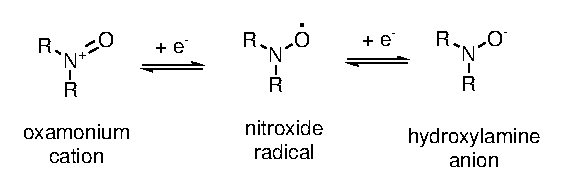
\includegraphics[width=.5\linewidth]{Figure1}
	\caption{Oxidized (left) and reduced (right) form of the the nitroxide radical (center).}
	\label{fig:states}
\end{figure}

\section{Theory}

\subsection{Redox potential of an ion in solution}

According to Ref.~\cite{marenichComputationalElectrochemistryPrediction2014}, the absolute reduction potential $E_{abs}^0$ (in \si{\volt}) of the half-reaction of reduction of $X^z$, $X^{z} + n_e\,e^- \rightarrow X^{z-n_e}$, reads: \begin{equation}
	E_{abs}^0(X^{z}|X^{z-n_e}) = -\frac{\Delta G_{r}^\star}{n_e\,F}, \text{ with } \Delta G_{r}^\star = G^\star(X^{z-n_e}) - G^\star(X^z), \label{eq:nernst}
\end{equation}
where $\Delta G_{r}^\star$ is the free Gibbs energy of the reduction reaction in solution, $F$ is the Faraday constant and $n_e$ the number of electrons involved in the reduction process. Last but not least, $G^\star(X^z)$ is the Gibbs free energy of $X^z$ in solution.  In the rest of this article, it is considered that $G^\star(e^-) = 0$.

From a phenomenological point of view, such energy is the sum of the one of the system in vacuum, plus the change in (free) energy resulting from its transfer to an electrolytic solution, \textit{i.e.}, $G^\star(X^z) = G^0(X^z)+ \Delta G_S^\star(X^z)$. The latter may be further decomposed using the thermodynamic cycle presented in Figure \ref{fig:th}. There are four steps: $\Delta G_d + \Delta G_s$ (discharge of a sphere in gas phase followed by charge in a dielectric) is a purely electrostatic processes, while $\Delta G_s$ is due, in most part, to non-electrostatic contributions (cavitation, vdW, etc). Finally, $\Delta G^\star_{DH}$ adds the effect of surrounding ions, and is therefore important to treat electrolytes \cite{silvaImprovingBornEquation2024}.

\begin{figure}[!h]
	\centering
	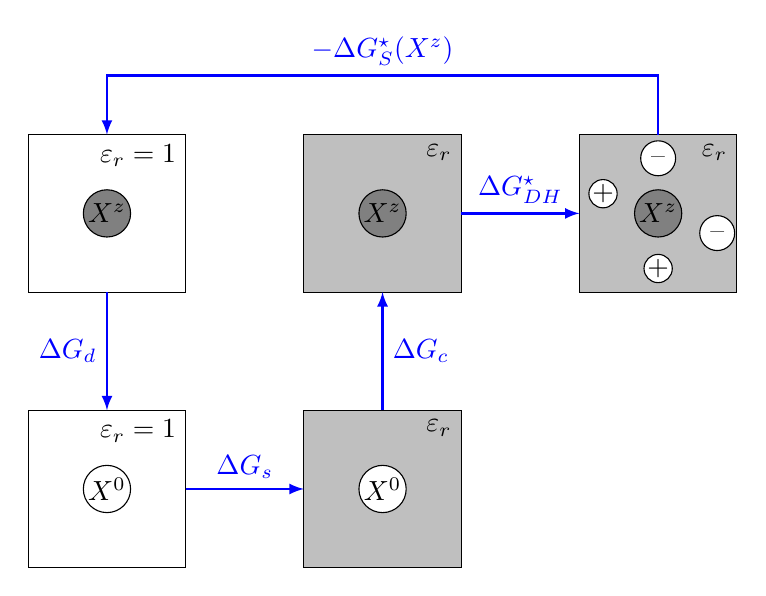
\begin{tikzpicture}
		\draw (-1,-1) rectangle +(2,2) node[anchor=north east]{$\varepsilon_r=1$};
		\draw[fill=gray] (0,0) circle (.3cm) node{$X^z$};
		
		
		\draw (-1,-4.5) rectangle +(2,2) node[anchor=north east]{$\varepsilon_r=1$};
		\draw (0,-3.5) circle (.3cm) node{$X^0$};
		
		
		\draw[fill=gray!50] (2.5,-4.5) rectangle +(2,2) node[anchor=north east]{$\varepsilon_r$};
		\draw[fill=white] (3.5,-3.5) circle (.3cm) node{$X^0$};
		
		
		\draw[fill=gray!50] (2.5,-1) rectangle +(2,2) node[anchor=north east]{$\varepsilon_r$};
		\draw[fill=gray] (3.5,0) circle (.3cm) node{$X^z$};
		
		
		\draw[fill=gray!50] (6,-1) rectangle +(2,2) node[anchor=north east]{$\varepsilon_r$};
		\draw[fill=gray] (7,0) circle (.3cm) node{$X^z$};
		\draw (2.8+3.5,-3.25+3.5) node[draw,fill=white,circle,inner sep=0]{+}
		(3.5+3.5,-2.8+3.5) node[draw,fill=white,circle,inner sep=.075cm]{--}
		(4.25+3.5,-3.75+3.5) node[draw,fill=white,circle,inner sep=.075cm]{--}
		(3.5+3.5,-4.2+3.5) node[draw,fill=white,circle,inner sep=0]{+};
		
		\draw[blue,thick,-latex] (0,-1) -- +(0,-1.5) node[midway,left]{$\Delta G_d$};
		\draw[blue,thick,-latex] (1,-3.5) -- +(1.5,0) node[midway,above]{$\Delta G_s$};
		\draw[blue,thick,-latex] (3.5,-2.5) -- +(0,1.5) node[midway,right]{$\Delta G_c$};
		\draw[blue,thick,-latex] (4.5,0) -- +(1.5,0) node[midway,above]{$\Delta G^\star_{DH}$};
		\draw[blue,thick,-latex] (7,1) -- ++(0,.75) -- node[midway,above]{$-\Delta G_S^\star(X^z)$} ++(-7,0) -- ++(0,-.75);
	\end{tikzpicture}
	\caption{Thermodynamic cycle to compute the energy of solvatation of an ion, $X^z$, in a electrolyte (solvent characterized by a $\varepsilon = \varepsilon_0\,\varepsilon_r$ dielectric constant and by a ``cloud'' of other ions). $\Delta G_d$ is the discharge of $X^z$ in gas phase, $\Delta G_s$ is the solvatation of $X$, $\Delta G_c$ is the charging of $X$ in $\varepsilon$, and $\Delta G^\star_{DH}$ is the addition of the other ions.}
	\label{fig:th}
\end{figure}


On the one hand, at the quantum chemistry (QC) level, the solvatation energy is generally treated implicitly, thanks to a self-consistent reaction field approach (SCRF) \cite{herbertDielectricContinuumMethods2021}: \begin{align}
	G^\star_{SCRF}(X) &= \Braket{\Psi|{\hat{H}+\frac{1}{2}\hat{R}}|\Psi} + G_{th}[\Psi] + G_{nonelst}(X) \nonumber\\
	&= E[\Psi] + G_{th}[\Psi] + \underbrace{G_{elst}[\Psi] + G_{nonelst}(X)}_{\Delta G^\star_{S,SCRF}(X)}, \label{eq:scrf}
\end{align}
where $\Psi$ is the wavefunction of $X$ (minimized under the application of $\hat R$, so not equal to the gas phase wavefunction), $\hat H$ is the electronic Hamiltonian, $\hat R$ is the reaction field operator (generally recognized to give rise to the electrostatic contribution to the solvation energy, $G_{elst}$), $G_{th}$ are the thermal contributions to the Gibbs free energy derived from thermostatistic analysis, and $G_{nonelst}$ is the non-electrostatic contributions (cavitation, dispersion, etc) to the solvation energy. Therefore, using the notation of Figure \ref{fig:th} (and assuming no change in the geometry of $X^z$), $ \Delta G^\star_{S,SCRF}(X^z) = \Delta G_d + \Delta G_s + \Delta G_{c}$.  

On the other hand, the Debye-Huckel (DH) theory provide another estimate of $\Delta G_{S}^\star$ \cite{bockrisModernElectrochemistryIonics1998}. Indeed, assuming that a ion $X^z$, bearing a charge $q = z\,e_0$ ($e_0$ is the elementary charge), can be approximated by a sphere of radius $a$ and that the ions in the solution are distributed in the solution according to Maxwell-Boltzmann statistics, one obtains the corresponding solvation energy as \cite{kontogeorgisDebyeHuckelTheoryIts2018,silvaDerivationsDebyeHuckel2022,silvaImprovingBornEquation2024}:\begin{align}
	\Delta G^\star_{S,DH}(X^z)
	&= \Delta G^\star_{born}(X^z) + \Delta G^\star_{DH}(X^z)\label{eq:adh}
\end{align}
where:
\begin{equation}
	\Delta G^\star_{Born}(X^z) =\frac{q^2}{8\pi\varepsilon_0\,a}\,\left[\frac{1}{\varepsilon_r}-1\right], \label{eq:born}\\
\end{equation}
and,
\begin{align}
	&\Delta G^\star_{DH}(X^z) = -\frac{q^2}{4\pi\varepsilon_0\varepsilon_r}\,\frac{\kappa}{(\kappa\,a)^3}\,\left[\ln(1+\kappa\,a)-\kappa\,a+\frac{1}{2}(\kappa\,a)^2\right],\label{eq:dh} \end{align}
in which $\kappa$ is the inverse of the Debye screening length, defined from:\begin{equation}
	\kappa^2 = \sum_i \frac{n_i\,q_i^2}{\varepsilon_0\varepsilon_r\,k_B\,T}, \label{eq:kappa2}
\end{equation}
where $n_i$ is the number density ($n_i = N_i / V = c_i\,\mathcal{N}_a$ where $\mathcal{N}_a$ is the Avogadro number and $c_i$ is the concentration in ion $i$) of ion of type $i$, $k_B$ is the Boltzmann constant, and $T$ is the temperature.  $\kappa$ is  proportional to the ionic strength of the solution, $I = \frac{1}{2}\sum_i c_i\,z_i^2$.  The Born part is generally dominant in solvatation energies predicted by this model (Fig.~S1).

In the limit of $\kappa\to 0$,  $\Delta G^\star_{DH} = 0$ and thus $\Delta G^\star_S \approx \Delta G^\star_{born} = \Delta G_d + \Delta G_c$.  Therefore, by combining Eqs.~\eqref{eq:scrf} and \eqref{eq:adh}, one defines:\begin{equation}
	G^\star(X^z) = G^\star_{SCRF}(X^z) + \Delta G^\star_{DH}(X^z), \label{eq:gtot}
\end{equation}
to be used in Eq.~\eqref{eq:nernst}. It should provide similar results to the approach developed by Cossi \emph{et al.} in Ref.~\citenum{cossiInitioStudyIonic1998}.

%

\subsection{Model for the ion-pair formation}

To further model the impact of the electrolyte on the redox potential, the formation of ion pairs is also considered (Fig.~\ref{fig:cip}).  Here, the electrolyte is composed of a pair \ce{AC}, where \ce{A-} and \ce{C+} are a cation and an ion, respectively.  Being favored by electrostatic interactions, the close-contact pairing of the oxidized (\ce{N+}) and reduced (\ce{N-}) state of nitroxide (\ce{N^.}) with its corresponding counterion (\ce{A-} and  \ce{C+},  respectively) is first considered. Then, further complexion with the \ce{AC} pair in close contact is considered  \cite{wylieImprovedPerformanceAllOrganic2019a}.

\begin{figure}[!h]
	\centering
	\newcommand{\arrwy}[3]{
		\draw [transform canvas={yshift=0.3ex},arrows = {-Stealth[harpoon]}] (#1) -- (#2) node[midway,above]{#3};
		\draw [transform canvas={yshift=-0.3ex},arrows = {-Stealth[harpoon]}] (#2) -- (#1);
		}
		\newcommand{\arrwx}[3]{
		\draw [transform canvas={xshift=0.3ex},arrows = {-Stealth[harpoon]}] (#1) -- (#2) node[midway,left]{#3};
		\draw [transform canvas={xshift=-0.3ex},arrows = {-Stealth[harpoon]}] (#2) -- (#1);
		}
	\begin{tikzpicture}[node distance=2cm]
		\node (N1) {\ce{N+ + A- + C+ + 2e-}};
		\node[right=1cm of N1] (N1c) {\ce{NA + C+ + 2e-}};
		\arrwy{N1.east}{N1c.west}{$K_{01}$}
		\node[left=1cm of N1] (N1cc) {\ce{NAC+ + 2e-}};
		\arrwy{N1cc.east}{N1.west}{$K_{02}$}
		
		\node[below of = N1] (N2) {\ce{N^. + A+ + C- + e-}};
		\arrwx{N1.south}{N2.north}{$K_{1}$}
		\node[below of=N1cc] (N2cc) {\ce{NAC^. + e-}};
		\arrwy{N2cc.east}{N2.west}{$K_{12}$}
		
		\node[below of=N2] (N3) {\ce{N- + A- + C+}};
		\arrwx{N2.south}{N3.north}{$K_2$}
		\node[right= 2cm of N3] (N3c) {\ce{NC  + A-}};
		\arrwy{N3.east}{N3c.west}{$K_{21}$}
		\node[below of=N2cc] (N3cc) {\ce{NAC-}};
		\arrwy{N3cc.east}{N3.west}{$K_{22}$}
	\end{tikzpicture}
	\caption{Scheme illustrating the different possible reactions: \ce{N+} and \ce{N-} are the oxidized and reduced forms of a given nitroxide, \ce{N^.}, and \ce{C+} and \ce{A-} are the countercation and anion coming from electrolyte, respectively. Horizontal arrows are ion-pairing reactions (with the i\ce{AC} pair in left, with a single counterion in right), while vertical arrows are electrochemical reactions.}
	\label{fig:cip}
\end{figure}

Assumptions:\begin{itemize}
	\item Redox process for ion pair is negligible (to be checked).
	\item $C_{\ce{N+}} = [\ce{N+}]+[\ce{NA}] + [\ce{NAC+}]$, etc.
	\item At equilibrium, $C_{\ce{N+}} = C_{\ce{N^.}}$, etc.
	\item at all time, $[\ce{A-}] = [\ce{C+}] = \ce[X]$ (electroneutrality)
\end{itemize}

xxx Nernst:\begin{align}
	E^f_{abs}(\ce{N+|N^.}) &= E^0_ {abs}(\ce{N+|N^.})+\frac{RT}{F}\,\ln\left[\frac{1+K_{12}\,[X]^2}{1+K_{01}\,[X]+K_{02}\,[X]^2}\right]\\
	E^f_{abs}(\ce{N^.|N-}) &= E^0_ {abs}(\ce{N^.|N-})+\frac{RT}{F}\,\ln\left[\frac{1+K_{21}\,[X]+K_{22}\,[X]^2}{1+K_{12}\,[X]^2}\right]
\end{align}
$K_{ij}= e^{-\frac{\Delta G_{ij}^\star}{RT}}$, where $\Delta G_{ij}^\star$ is the free Gibbs energy [computed with Eq.~\eqref{eq:gtot}] change for a given complexation reaction.

\section{Methodology}

\begin{itemize}
	\item the systems (Fig.~\ref{fig:nitroxides}), plus the electrolytes that were considered.
	\item $a$ computed as the largest distance between two atoms in the system
	\item Absoliute to relative potentials
\end{itemize}

\begin{figure}[!p]
\centering
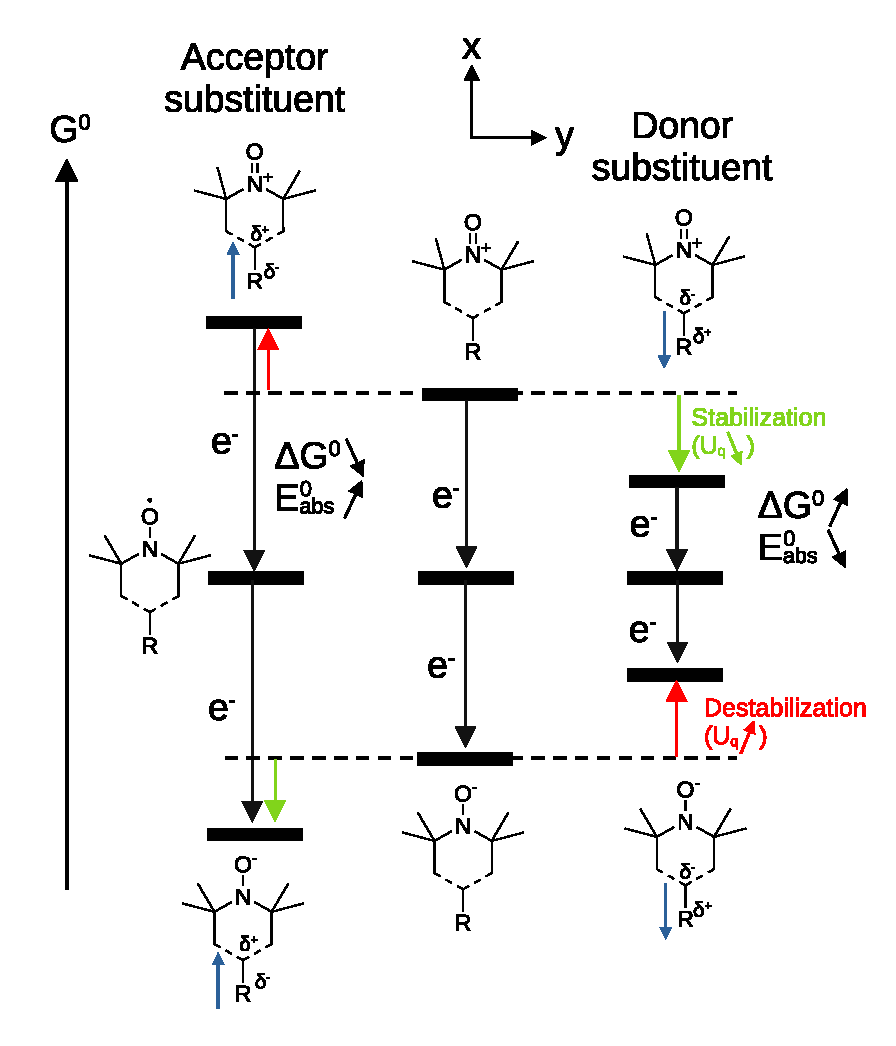
\includegraphics[width=\linewidth]{Figure4}
\caption{The different nitroxides considered in this work, sorted by families. Compounds \textbf{1}-\textbf{54} are from Ref.~\citenum{hodgsonOneElectronOxidationReduction2007}, while compounds \textbf{55}-\textbf{61} where considered for completeness. Experimental (reduction or oxidation) potentials are available in water if the number is written in red, while they are available in acetonitrile if the number is underlined.}
\label{fig:nitroxides}
\end{figure}

Geometry optimizations and subsequent vibrational frequency calculations were performed at the $\omega$B97X-D/6-311+G(d) level in water (described using the SMD \cite{marenichUniversalSolvationModel2009} approach) with Gaussian 16 C02 \cite{g16}. For compound \textbf{1}-\textbf{54}, the geometries obtained by Hodgson et al. \cite{hodgsonOneElectronOxidationReduction2007} have been used as a starting point, taking advantage of their extensive conformational search. All radical forms are considered to have a doublet ground state. Then, the compounds for which there are experimental redox potentials available in acetonitrile (see Figure \ref{fig:nitroxides}), geometry optimization and vibrational frequency calculations were also performed in this solvent. 

In this work, a value of $\varepsilon_r=80$ ($\varepsilon_r=35$ ) is used for water (acetonitrile). These relative permitivities are the one of pure solvent, and are known to be lower in corresponding electrolytes \cite{silvaTrueHuckelEquation2022}. These variations can be, indeed, quite substantial (for example, $\varepsilon\approx 70$ for a solution containing \SI{1}{\mol\per\kilo\gram} of \ce{NaCl} in water \cite{kontogeorgisDebyeHuckelTheoryIts2018,silvaTrueHuckelEquation2022}), but they are also strongly dependent on the nature of the electrolyte.

\section{Results and discussion}

\begin{itemize}
	\item Structure-activity relationships, on simple results (Figs.~\ref{fig:family}, \ref{fig:corr}), if possible (see Hodgson et al \cite{hodgsonOneElectronOxidationReduction2007}). Also, comparing water and acetonitrile (Fig.~\ref{fig:watvsac}).
	\item low-concentration limit: DH corrections (Fig.~\ref{fig:DH}).
	\item High-concentration limit: CIP (also, structure-activity relationship for CIP!, see Figs.~\ref{fig:Kx1} and \ref{fig:Kx2}) and Matsui.
	\item Comparison to experiment
\end{itemize}

\subsection{Structure-activity relationships}

Oxidation and reduction potentials of the nitroxide radicals in water, grouped by family, are plotted in Fig.~\ref{fig:family}. In comparison to \textbf{1}, changing the molecular structure or adding substituent generally increase both the oxidation and reduction potentials. Concerning the impact of the structure, 6-members ring compounds (P6O and APO)  display larger reduction potentials than their 5-members ring counterparts (P5O and  IIO), while adding one or two (IIO and APO) aromatic rings increase both the oxidation and reduction potential. 

\begin{figure}[!h]
	\centering
	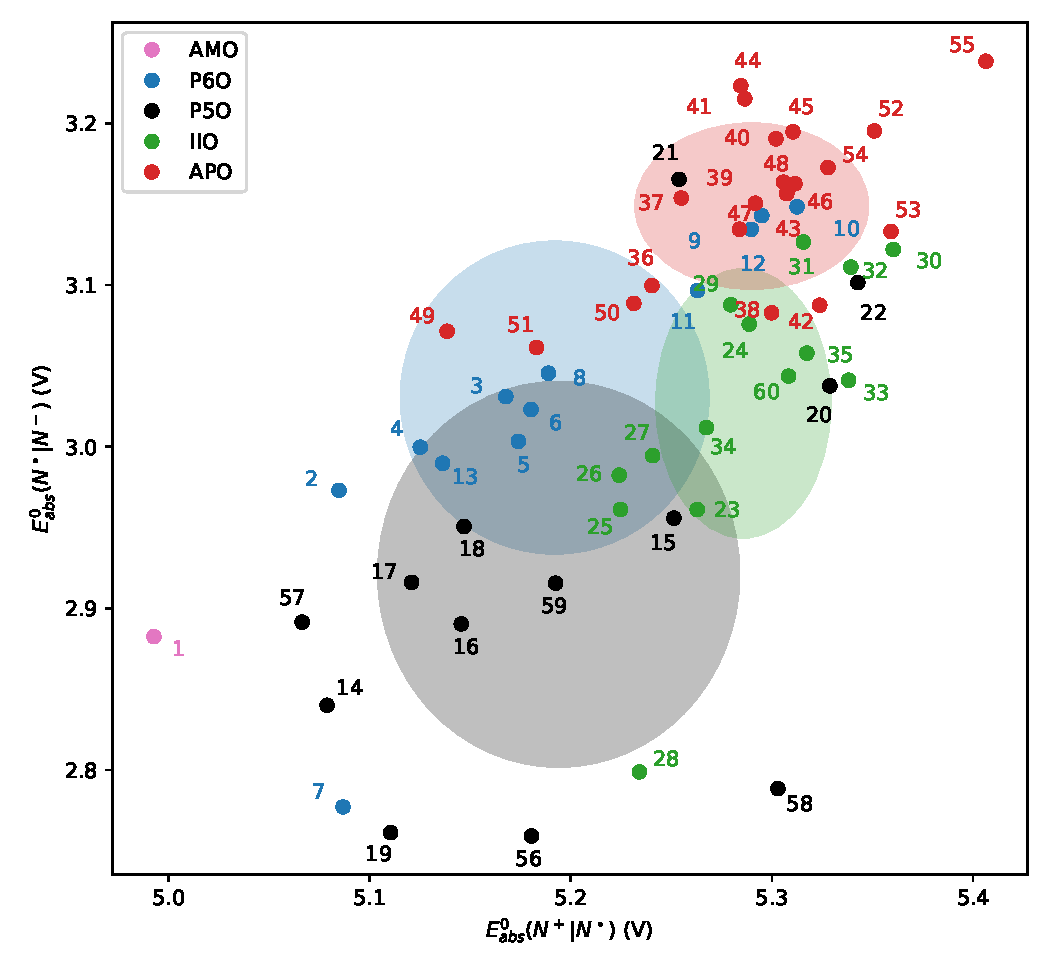
\includegraphics[width=.9\linewidth]{Figure5}
	\caption{Relationship between absolute oxidation and reduction potentials of nitroxides, as computed at the $\omega$B97X-D/6-311+G(d) level in water (SMD), with $[\ce{X}]=\SI{0}{\mole\per\liter}$. The color indicate the family (Fig.~\ref{fig:nitroxides}). For each of them, an ellipse is drawn, centered on the mean potential value among the family, and which width and height are given by the standard deviations.}
	\label{fig:family}
\end{figure}

Concerning the impact of the substituent, one can first notice than non-substituted nitroxides of each family (\textit{i.e.}, \textbf{2}, \textbf{14}, \textbf{23}, and \textbf{36}) have generally one of the lowest oxidation and reduction potential inside their group. Some trend also exists depending on the nature of the substituent: \begin{inparaenum}[(i)]
	\item shielding the radical center with ethyls instead of methyls (\textbf{7}, \textbf{19}, and \textbf{28}) results in a decrease of the potentials (especially the reduction), probably due to the change in inductive character, 
	\item  protonating \ce{NH2} increases the potentials, especially in P5O,
	\item multiple substitutions by COOH (\textit{e.g.},  \textbf{8} vs \textbf{9} and \textbf{10}) also increases the potentials, though less in IIO and APO, 
	\item mesomeric donors (\ce{NH2}, \ce{OH}, \ce{OMe}) substituted compounds have lower potentials than acceptor substituted ones (COOH, \ce{NO2}), especially in aromatic systems (IIO and APO).
\end{inparaenum}
As a consequence, \textbf{55} have the largest oxidation and reduction potential of all the compounds studied in this paper.

Following previous attempts, to explain these effects, correlation of both potentials with Hammet constants have been attempted for P5O and P6O but turns out very weak, especially for the reduction (Fig.~S2). In 2018, another model have been proposed by Zhang \textit{et al} \cite{zhangEffectHeteroatomFunctionality2018} in which change in oxidation potential is explained by the electrostatic interaction between the substituent(s) and the charge formed upon oxidation ($>$\ce{N+=O}). Said interaction may be expanded in as a  multipole expansion, which they proposed to truncated after the quadrupole term ($Q$),\begin{equation*}
	E_r(r) = \frac{\mu_x}{r^2} + \frac{Q_{xx}}{r^3},
\end{equation*}
assuming a non-charged substituent. The different quantities (dipole moment, $\mu_x$, and traceless quadrupole moment, $Q_{xx}$) are evaluated through a single point calculation at the same level of approximation [here, $\omega$B97X-D/6-311+G(d)] in gas phase on a simplified structure, using the geometry of the radical but where the $>$\ce{N-O^.} moiety is substituted by \ce{CH_2} (the rest of the geometry is kept fixed). This geometry is oriented so that the $x$ axis pass through the nitrogen and the atom (P6O, APO) or the center of the bond (P5O, IIO) that is further away in the ring, $r$ being the distance between these two points. Results are given in Fig.~\ref{fig:corr}. 

\begin{figure}[!h]
\centering
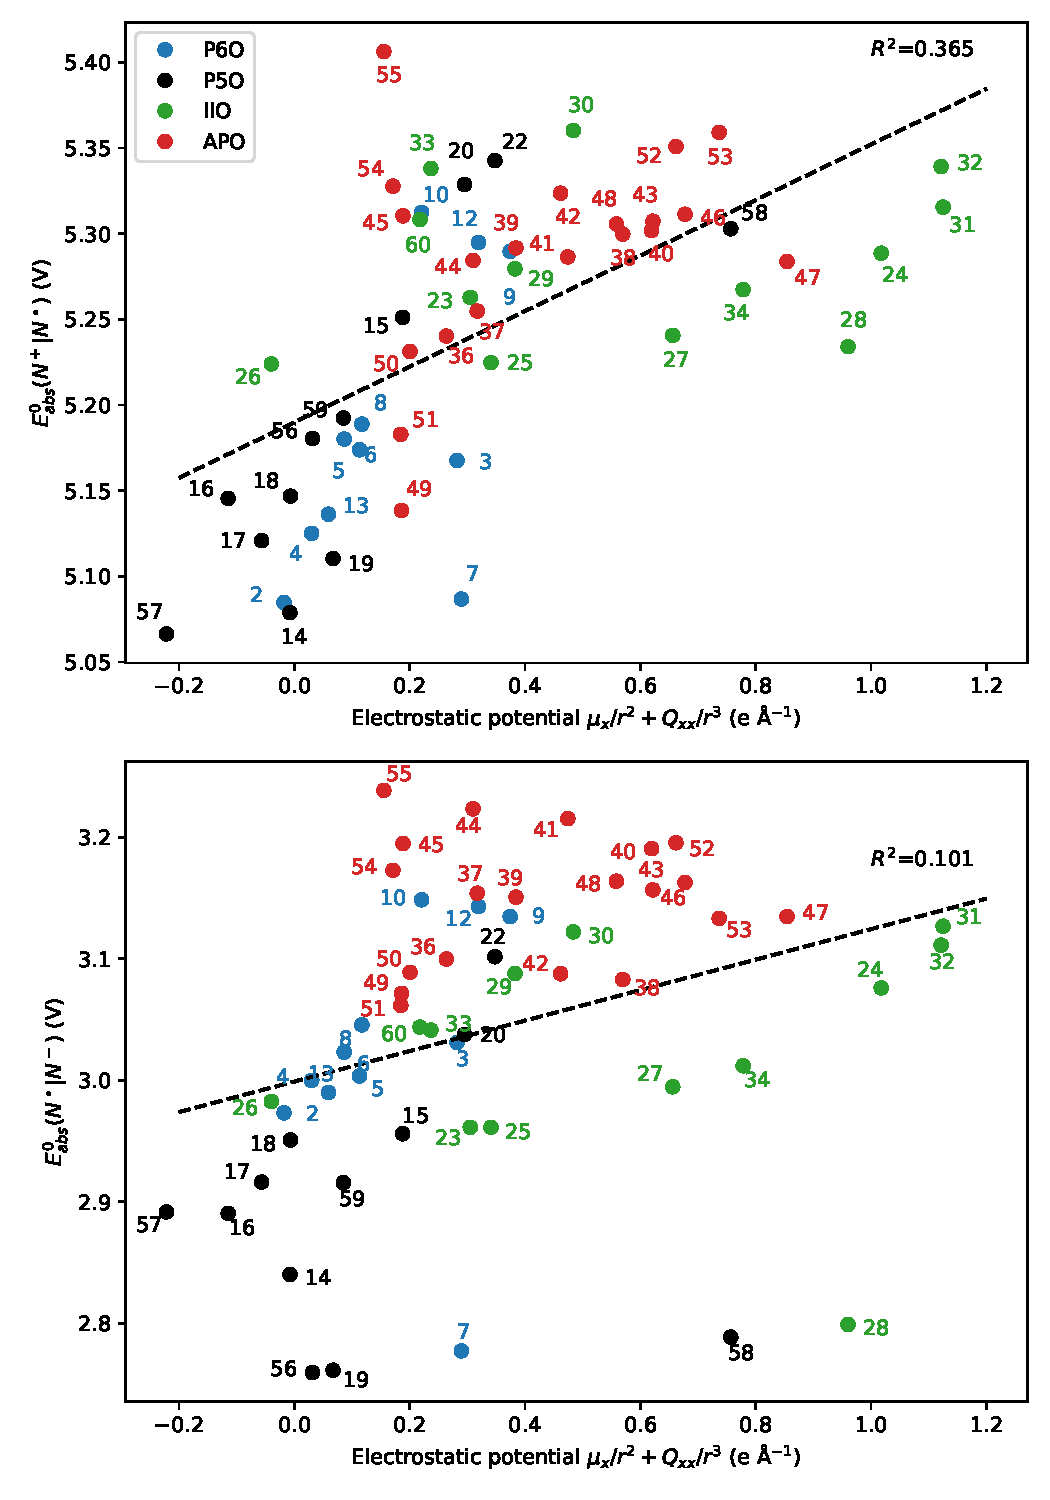
\includegraphics[width=.9\linewidth]{Figure6}
\caption{Relationship between absolute oxidation (top) and reduction (bottom) potentials of nitroxides and the electrostatic potential between the redox center ($>$\ce{N-O^.}) and the substituent, as computed at the $\omega$B97X-D/6-311+G(d) level in water (SMD), with $[\ce{X}]=\SI{0}{\mole\per\liter}$. Triangular marker ($\blacktriangle$) indicates results that are excluded from the correlation (see text).}
\label{fig:corr} 
\end{figure}

While this model fails to account for the effect of the substitution of methyls in ethyls  or to explain the modification due to disubsitutents, it results in an acceptable ($R^2 = 0.55$) correlation with the oxidation potential when the aformentioned molecules are removed (the correlation with the reduction potential remains, however, weak). It thus helps in explaining some the effect mentioned above: on the one hand, the increase in oxidation (and reduction) potential for aromatic compounds is correlated with an increase in quadrupole moment while, on the other hand, the modification due to donor/acceptor substituents are linked to change in the dipole moment. Another strength of this model is that while it is not applicable \textit{per se} to charged substituent (the multipole moment are ill-defined in that case), the leading term $q/r$ would result in a positive of $E_r$, well correlated with the change in oxidation and reduction potential mentioned above. One should note, however, that the changes due to the position of the substituent on the molecule are also not addressed by this model, which may explain the poor correlation for the reduction potential.

\subsection{Impact of the solvent}

\begin{figure}[!h]
	\centering
	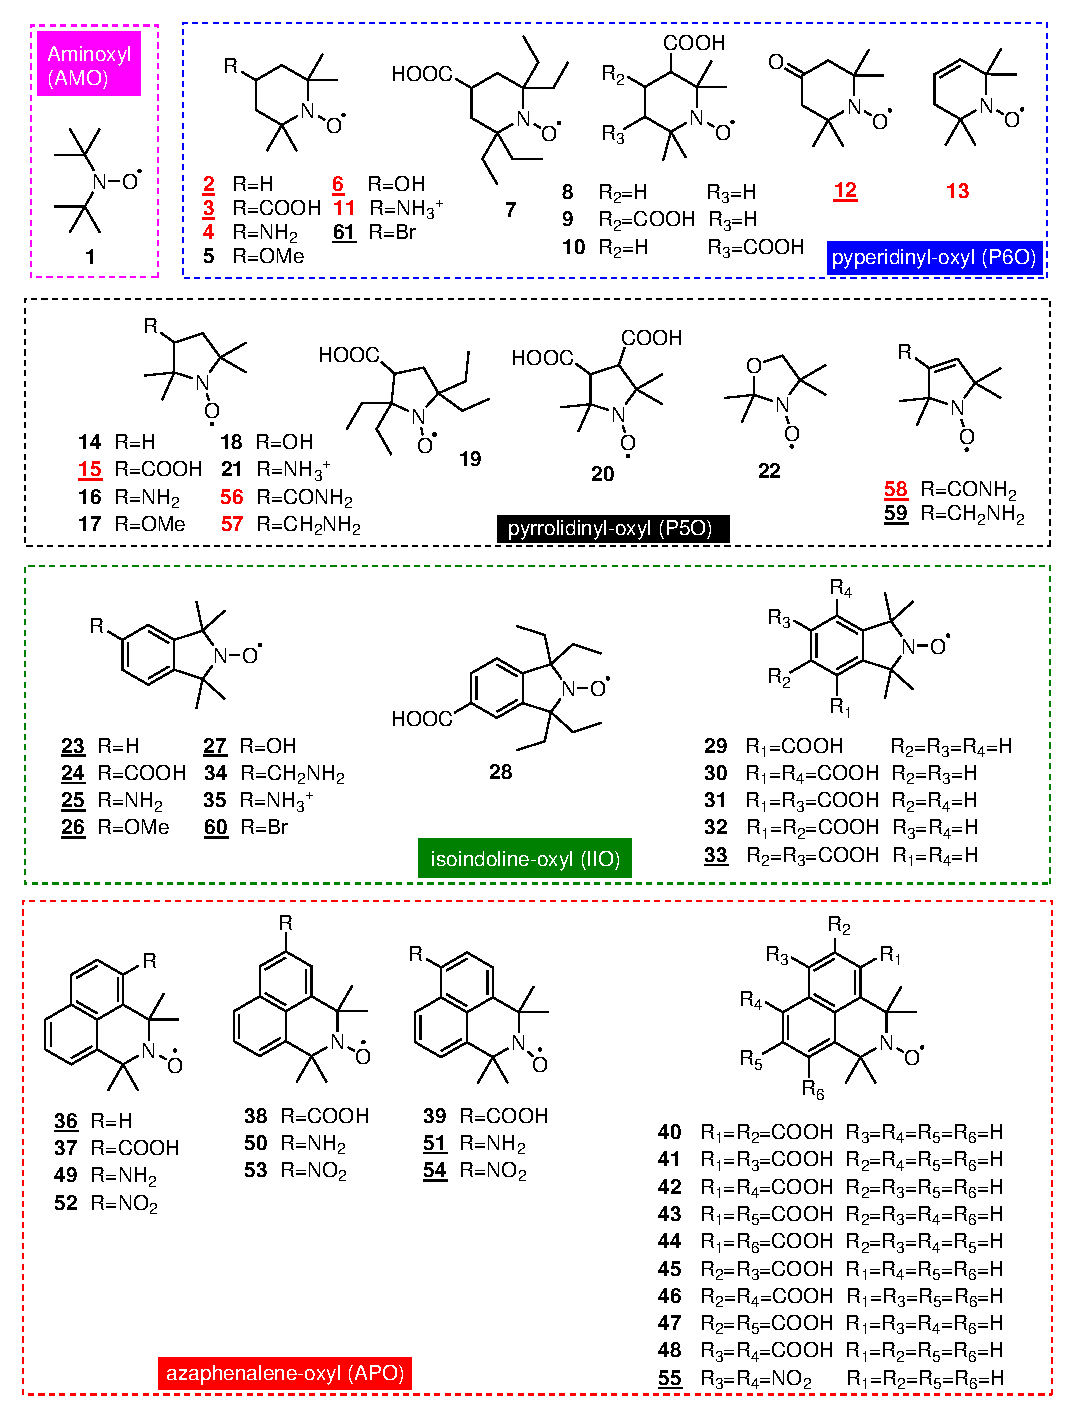
\includegraphics[width=\linewidth]{Figure7}
	\caption{Comparison between absolute oxidation (left) and reduction (right) potentials of nitroxides as computed at the $\omega$B97X-D/6-311+G(d) level in water and acetonitrile (SMD), with $[\ce{X}]=\SI{0}{\mole\per\liter}$. The dashed line represents no change. }
	\label{fig:watvsac}
\end{figure}


\begin{figure}[!h]
	\centering
	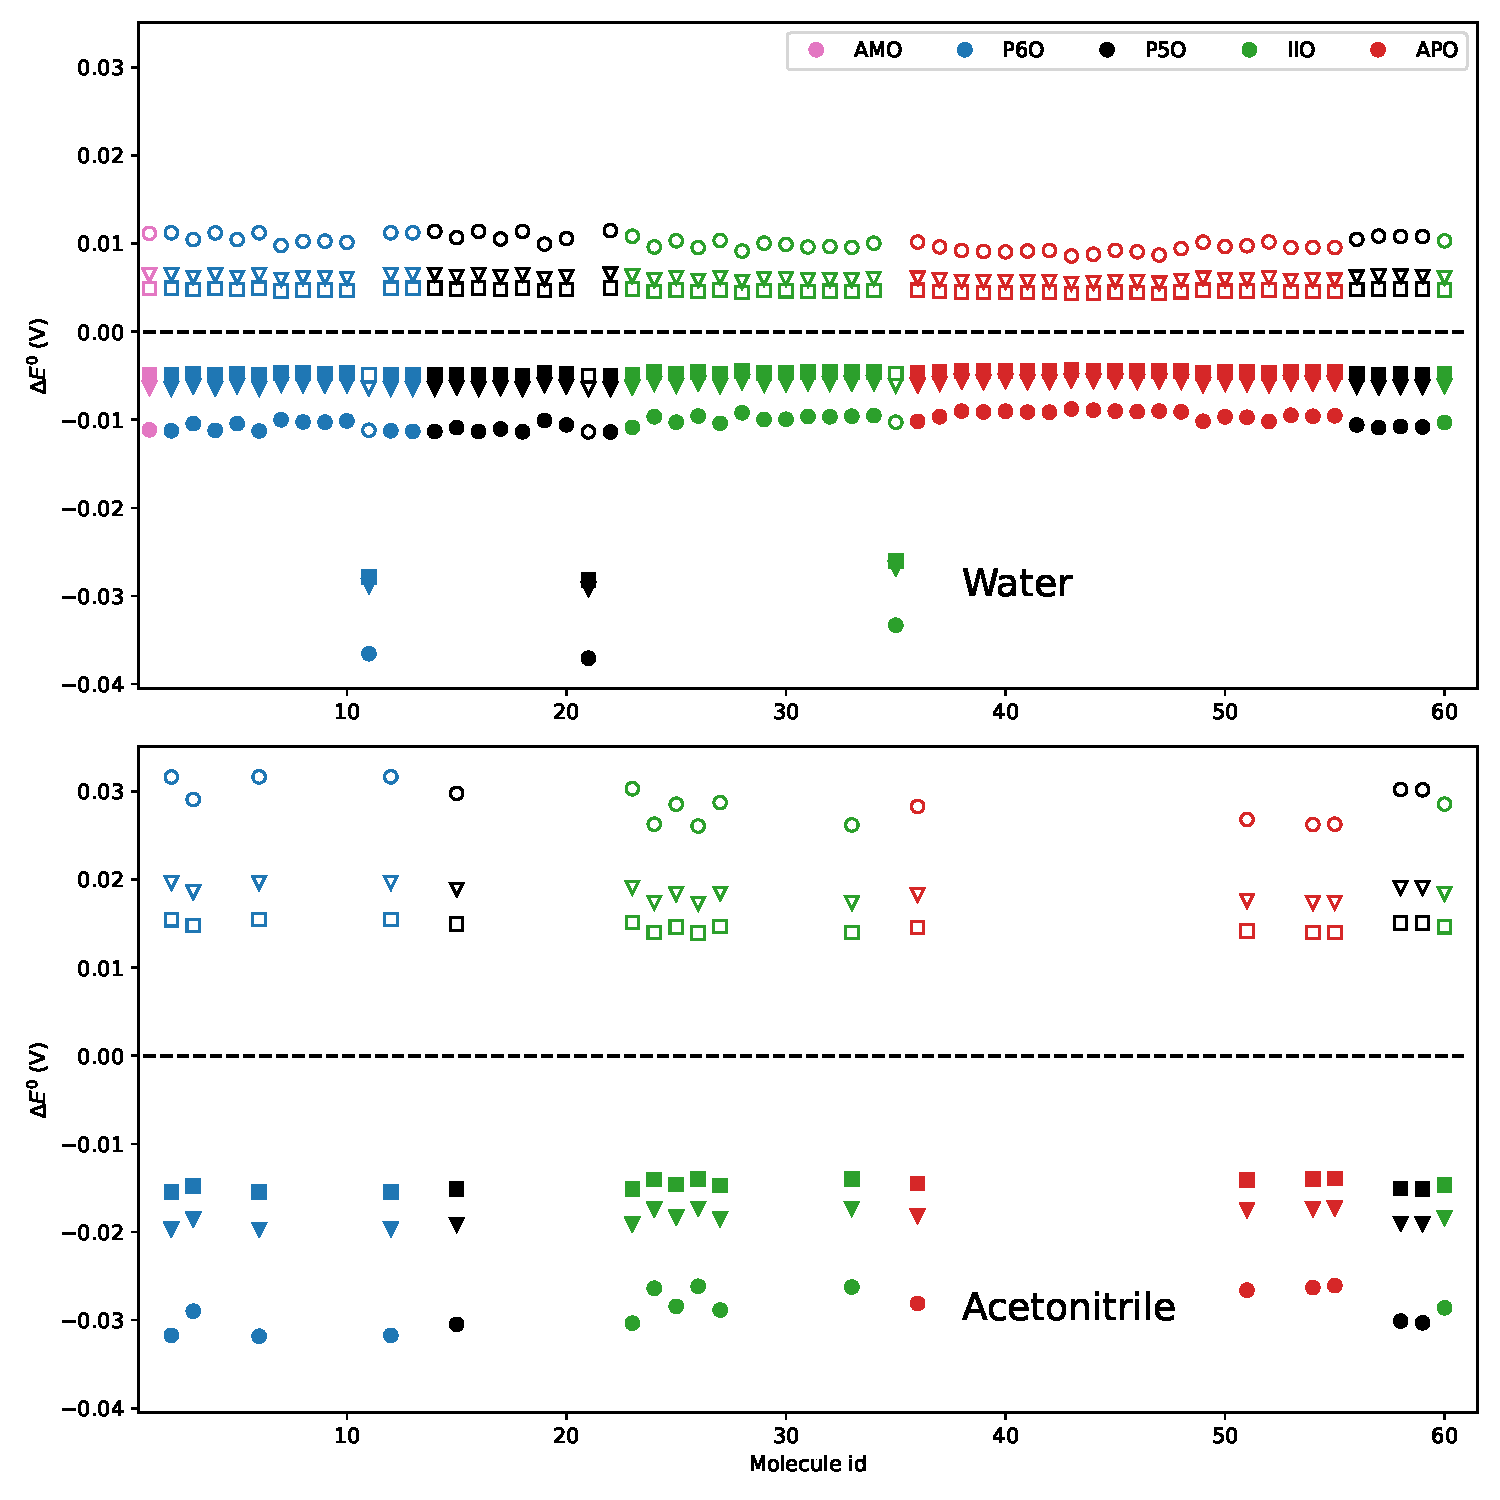
\includegraphics[width=\linewidth]{Figure8}
	\caption{Impact of the Debye-Huckel correction, as $\Delta E^0 = -\frac{\Delta G_{DH}^\star}{F}$ for $[X]=\SI{1}{\mole\per\liter}$ (round markers), $[X]=\SI{0.1}{\mole\per\liter}$ (triangular markers, $\blacktriangle$)  and $[\ce{X}]=\SI{0}{\mole\per\liter}$ (square markers, $\blacksquare$), as computed at the $\omega$B97X-D/6-311+G(d) level in water (top) and acetonitrile (bottom) using SMD. Filled (empty) markers represent the correction to the oxidation (reduction) potential. }
	\label{fig:DH}
\end{figure}


\begin{figure}[!h]
\centering
\includegraphics[width=\linewidth]{Figure9}
\caption{Value of the complexation equilibrium constants $K_{01}$ (round markers, $\bullet$) and $K_{21}$ (square markers, $\blacksquare$) for the 3 oxidation state of nitroxides, as computed at the $\omega$B97X-D/6-311+G(d) level in water (top) and acetonitrile (bottom) using SMD and $[X]=\SI{1}{\mole\per\liter}$.  The dashed line is there to help visualization. }
\label{fig:Kx1}
\end{figure}


\begin{figure}[!h]
\centering
\includegraphics[width=\linewidth]{Figure10}
\caption{Value of the complexation equilibrium constants $K_{02}$ (round markers, $\bullet$), $K_{12}$ (triangular markers, $\blacktriangle$) and $K_{22}$ (square markers, $\blacksquare$) for the 3 oxidation state of nitroxides, as computed at the $\omega$B97X-D/6-311+G(d) level in water (top) and acetonitrile (bottom) using SMD and $[X]=\SI{1}{\mole\per\liter}$.  The dashed line is there to help visualization. }
\label{fig:Kx2}
\end{figure}

\section{Conclusion}

Well.
	
	
\bibliographystyle{elsarticle-num-names} 
\bibliography{biblio}
	
\end{document}
\endinput
%%
%% End of file `elsarticle-template-num.tex'.
